\documentclass[twocolumn]{article}

\usepackage{minted}
\usepackage{graphicx}
\usepackage{titlesec}
\usepackage[english]{babel}
\usepackage{enumitem}
\usepackage[hmarginratio=1:1,top=32mm,columnsep=20pt]{geometry}
\usepackage[bottom]{footmisc}
\usepackage[hidelinks]{hyperref}
\usepackage{amsmath}
\usepackage{amssymb}
\usepackage{amsthm}
\usepackage{fixme}
\usepackage{xcolor}
\usepackage{subcaption}
\usepackage{cite}

\usepackage{tikz}
\usetikzlibrary{shapes,arrows}

\tikzstyle{block} = [rectangle, draw, fill=orange!20, text width=5em, text centered, minimum height=3em]
\tikzstyle{line} = [draw, -latex']
\tikzstyle{cloud} = [draw, ellipse,fill=red!20, node distance=3cm, minimum height=3em]

% FIXME Setup
\fxsetup{
  status=draft,
  author=,
  layout=inline,
  theme=color
}
\definecolor{fxnote}{rgb}{0.8000,0.0000,0.0000}
\colorlet{fxnotebg}{yellow}
\makeatletter
\renewcommand*\FXLayoutInline[3]{%
  \@fxdocolon {#3}{%
    \@fxuseface {inline}%
    \colorbox{fx#1bg}{\color {fx#1}\ignorespaces #3\@fxcolon #2}}}
\makeatother

\renewcommand\thesection{\Roman{section}}
\renewcommand\thesubsection{\alph{subsection}}
\titleformat{\section}[block]{\large\scshape\centering}{\thesection.}{1em}{}
\titleformat{\subsection}[block]{\large}{\thesubsection.}{1em}{}

\setlist[itemize]{noitemsep}
\setlist[enumerate]{noitemsep}

\newcommand{\ts}[1]{\mintinline{typescript}{#1}}
\newcommand{\hs}[1]{\mintinline{haskell}{#1}}

\newcommand{\fcy}[1]{\mathcal{#1}}
\newcommand{\lit}[1]{\text{``#1''}}
\newcommand{\etag}[1]{\textsf{#1}}

\newcommand{\ff}[1]{\textsf{#1}}

\newtheorem{theorem}{Theorem}

\title{Typed Interactions for NLU in Opal}
\author{Harrison Goldstein}
\date{Fall 2017}

\begin{document}
\maketitle

\begin{abstract}
  Natural Language Understanding (NLU) is a powerful tool for modern
  applications. Interacting with remote NLU engines can be error prone: most
  backends provide no type guarantees, and configuration synchronization is a
  constant source of bugs. We present a DSL for configuring a NLU application
  that ensures synchronization and type-safety.
\end{abstract}

\section{Introduction} \label{introduction}
In the 1970's, a text-based command interface was ``good enough'' for people
interacting with computers. After all, most of the computation being done was
fairly specific to some application domain, the person operating the computer
was well-trained, and the machine was viewed as a tool for getting the job done.

Today, computers are our personal assistants. They are integrated with our lives
and they help everyday people do everyday tasks. Most people who use computers
today never touch a command shell, and even those who do would often rather not.
Graphical interfaces are amazingly powerful, and are often sufficient to allow
users to easily interact with the computer, but even those have their drawbacks.
We would really like our personal assistant to respond to commands in human
language:
\begin{itemize}
\item ``Hey Siri! Play some music.''
\item ``Ok Google. Navigate to my hotel.''
\item ``Slackbot, set my status to active.''
\end{itemize}
This is the realm of Natural Language Understanding (NLU).\footnote{We do not
  distinguish between spoken or written language when talking about NLU in
  general.}

We have seen a huge growth in NLU applications in recent years, and we will
likely see more. Unfortunately, there has been no serious effort made to make
this power available at the language level, so programmers have been forced to
integrate these technologies into their applications by hand. We propose an
addition to the Opal language that will begin to close this
gap.\cite{opal-arxiv}

\subsection{An Example}
Consider a simple \emph{reminders} interface to a calendar or other scheduling
assistant. A user might ask the application to set a reminder containing a
message and a time (for simplicity, we will just allow the user to specify
\ts{later} or \ts{tomorrow}) or she might ask the application to get any active
reminders. Since Opal is embedded in TypeScript,\cite{typescript} a typical Opal
application might express this interface with the following declarations:
\begin{minted}{typescript}
  type Msg = string;
  type Time = "later" | "tomorrow";
  type Set = {
    msg: Msg,
    time: Time
  };
  type Intent =
    | { tag: "Set", data: Set }
    | { tag: "Get", data: {} };
\end{minted}

We would like to interact with this application via human language, so we need
some way of converting a user's \emph{utterance} to something of type
\ts{Intent}. Figure \ref{fig:drycleaning} shows the desired data representation
of a user utterance.

\begin{figure}
\begin{minted}{typescript}
  {
    tag: "Set",
    data: {
      msg: "pick up the dry cleaning",
      time: "later",
    }
  }
\end{minted}
  \caption{The desired data representation of the utterance: \emph{Remind me
      later to pick up the dry cleaning}.}
  \label{fig:drycleaning}
\end{figure}

\subsection{Types for NLU}
If a programmer simply wrote down types like the ones above, set up their NLU
engine, and started their application, there would be a problem. Since there is
no connection between the types and the NLU configuration, these types could
actually be unsound! If the programmer made a mistake in \emph{either} the types
\emph{or} the configuration, the application would be unusable and no compiler
could possibly know. Bugs like these are particularly insidious because they
might be mistaken as network errors or even just as an indicator of
under-training.

In this work, we set out to connect the types and the NLU configuration,
allowing the programmer to avoid these awful bugs. There are a few ways that one
might try to do this. First, the programmer could write down the NLU
configuration and extract the types from it. This is pretty much a non-starter,
since there is fundamentally less information in the NLU configuration than
there is in the type definitions. Instead, the programmer could write the types,
and extract the NLU information from those. This approach is more feasible, but
it would require some kinds of annotations in the types to capture
implementation-specific properties of the configuration.

We present a third option: a domain specific language (DSL) for simultaneously
specifying
\begin{itemize}
\item configuration for an NLU engine;
\item a typed interface for responses
\end{itemize}
This allows the user to tune the configuration as much as they need, to write
useful types, and to ensure that these two artifacts are always compatible.
\\

We will begin by presenting a technical description of our type language in
Section \ref{description}. In Section \ref{formalism}, we present a formal
specification for the language our type-directed response parsing algorithm.
Section \ref{implementation} covers the implementation of the language and
related libraries. Finally, Sections \ref{evaluation} and \ref{future} present
an evaluation of our work, and our plans for future work, respectively.

\section{Language Description} \label{description}
For our initial work, we elected to focus on building a system to support a
single NLU backend---specifically, we are working with an NLU engine called
Wit.\cite{wit} When configuring Wit, as with many NLU backends, the main task is
setting up the \emph{entities} that Wit should be looking for. An entity is a
discrete piece of information that the NLU engine extracts from an utterance. In
our example, the messages and the time are both entites, as is the user's
intent.

\subsection{Search Strategies}
When entities are declared, the user must specify a ``search strategy.'' In the
case of Wit, there are three main strategies:
\begin{description}
\item[Free Text] Entities that are found via free text matching are just strings
of text from the utterance. In our example, the message is a free text entity.
\item[Keywords] Keywords entities are just words from some pre-defined set.
  Things like \ts{later} and
  \ts{tomorrow} would be captured via keyword searching.
\item[Trait] These are slightly more abstract. Traits capture something that is
  a quality of the utterance as a whole. Something like a user's intent or even
  their mood could be a trait.
\end{description}

To some, these lookup strategies might seem like an implementation detail, but
there is actually something important going on here. The search strategies are
closely tied to the \emph{type} of the desired output. In the case of free text
and keywords, this association is obvious: free text entities are just
\ts{string}s, and keywords are members of a union of literal
types.\footnote{For example, \texttt{"later" | "tomorrow"}.} Traits are slightly
more complex, but they essentially represent a tagged union, where the extracted
entity itself carries only the tag. We will make these ideas more concrete in
section \ref{formalism}.

\subsection{The DSL}
With our observations about search strategies in mind, we can write our types
from before in a slightly different way. Figure \ref{fig:dsl_decls} shows the
same type declarations from Section \ref{introduction} written in our DSL.

\begin{figure}
\begin{minted}{typescript}
  free-text Msg
  keywords Time = "later" | "tomorrow"
  alias Set = {
    msg: Msg,
    time: Time
  }
  trait Intent =
    | <Set> Set
    | <Get> {}
\end{minted}
  \caption{Some DSL declarations.}
  \label{fig:dsl_decls}
\end{figure}

The main thing to notice is that the keyword \ts{type} has been replaced by
entity declarations \ts{free-text}, \ts{keywords}, and \ts{trait}, or by
\ts{alias}. There are a number of benefits of entity declarations. First and
foremost, it allows the user to explicitly define the NLU engine configuration
alongside the program types. With types defined in our DSL, we can automatically
generate configuration for entities that is guaranteed to be consistent with the
types in the program. When a \ts{Time} is returned to the user, it will be
guaranteed to be either \ts{"later"} or \ts{"tomorrow"}. This alone solves a lot
of the problems that tend to come up when writing these types of applications.

Another benefit of these bespoke declaration forms is simplified syntax. When a
\ts{free-text} entity is declared, there is no need to write ``\ts{= string},''
because that is implied by the search strategy. Similarly, since traits are
always tagged unions, we can write them in (almost) ML syntax, rather than
writing out the standard TypeScript workaround.

Finally, writing specific entity declarations rather than just \ts{type}, makes
it clear that there is more going on than a direct translation into TypeScript.
In fact, the DSL parser does lot of validation to guarantee that only reasonable
types can be written down. For example, a \ts{keywords} declaration is required
to be a union, and that union must contain only literals. Even the \ts{alias}
keyword has some validation built in. Some TypeScript types would be problematic
if they were allowed---we enforce those conditions in the DSL.

\begin{figure}
  \centering
  \begin{align*}
    \mathbb{D} ::=&\ \text{FreeText}(\etag{t}) \\
    |&\ \text{Keywords}(\etag{t},\ [\ell]) \\
    |&\ \text{Trait}(\etag{t},\ \{s: \mathbb{T}\}) \\
    |&\ \text{Alias}(\etag{t},\ \mathbb{T}) \\
    \\
    \mathbb{T} ::=&\ \text{Def}(\etag{t}) \mid \ell \mid \{s: \mathbb{T}\}
  \end{align*}
  $$ \etag{t} \in \ff{Tag} \qquad \ell, s \in \textbf{string} $$
  \caption{The abstract syntax tree for our DSL.}
  \label{fig:ast}
\end{figure}

Figure \ref{fig:ast} shows the AST that is produced when we parse the DSL.
Looking at this, it also becomes clear that the limitations on the types allowed
in a trait declaration are fairly strict. As of writing, there are only three
types allowed within a trait declaration: previously defined declarations,
literals, and records (where each element is subject to the same restrictions).
These limitations match up with the capabilities of NLU engines in general.
While many backends provide the ability to parse numbers, dates, and other data,
these types of entities are implementation specific. In Section \ref{future}, we
discuss plans to expand the allowed types in a modular way.

\subsection{NLU Engine Responses}
Our DSL solves quite a few problems on its own. It forces the program types to
agree with the NLU configuration, and it provides a convenient way to write both
down together. It also prevents the user from having unreasonable expectations
of the backend, by restricting the types that a user can expect as a response.

Unfortunately, there is still one major issue. The vast majority of NLU engines
do not return structured data. Instead, they return a bag of entities with no
information about the relationships between them. Figure \ref{fig:nostructure}
shows a sample response. Recall that in our example, \ts{Msg} and \ts{Time}
entities were only expected when there was an \ts{Intent} with tag \ts{"Set"}.
Furthermore, our types dictate exactly where in the data structure those entity
values should end up. The popular libraries, Wit incuded, igore this structure
entirely.

\begin{figure}
\begin{minted}{typescript}
  {
    Intent: ["Set"],
    Msg: ["pick up the dry cleaning"],
    Time: ["later"]
  }
\end{minted}
  \caption{The unstructured response for the utterance: \emph{Remind me later to
      pick up the dry cleaning}.}
  \label{fig:nostructure}
\end{figure}

This makes it necessary to have a run-time component of the system that knows
how to reconstruct structured data from the unstructured response that comes
from the NLU engine. Building structured data from the response is a nontrivial
task. First, it requires that information about the relationships between
entities and data be available at run-time. This is mostly an engineering
problem, and our solution is outlined in Section \ref{implementation}.

The other difficulty is that the types might admit more than one valid response
object. To see how this works, imagine that we want to allow a user to set two
messages at once. We would change the \ts{Set} type to be:
\begin{minted}{typescript}
  type Set = {
    msg1: Msg,
    msg2: Msg,
    time: Time
  };
\end{minted}
Unfortunately, this kind of ambiguity makes it impossible to find a principled
way of parsing a response. Since the backends do not expose ordering
information, a response with two \ts{Msg} fields might parse to any of four
different objects. We say four because the reconstruction algorithm might
reasonably ignore one of the messages and just put the same one for \ts{msg1}
and \ts{msg2}. For this reason, we impose the restriction that declarations do
not reuse entities.

\section{Formalism} \label{formalism}
In order to reason about the correctness of our translations, we have formalized
the results from Section \ref{description}. We begin by writing down a core
language for the type DSL as shown in Figure \ref{fig:grammar_a}.
\begin{figure}
  \centering
  \begin{subfigure}{1\linewidth}
    \begin{align*}
      \fcy{D} ::=&\ \text{FreeText}(\etag{t}) \\
      |&\ \text{Keywords}(\etag{t},\ [\ell]) \\
      |&\ \text{Trait}(\etag{t},\ \{s: \fcy{T}\}) \\
      \\
      \fcy{T} ::=&\ \fcy{D} \mid \ell \mid \{s: \fcy{T}\}
    \end{align*}
    $$ \etag{t} \in \ff{Tag} \qquad \ell, s \in \textbf{string} $$
    \caption{The core language.}
    \label{fig:grammar_a}
  \end{subfigure}\vspace{1cm}
  \begin{subfigure}{1\linewidth}
    $$ \tau ::=\ \textbf{string} \mid \ell \mid \{s: \tau\} \mid \langle \tau
    \rangle $$
    \caption{Opal types.}
    \label{fig:grammar_b}
  \end{subfigure}
  \caption{Formal structures.}
\end{figure}
There are similarities between these definitions and the ones in Figure
\ref{fig:ast}, but the core language has some slightly different goals. First,
we remove aliases and require that all type definitions are written ``in-line.''
Next, rather than split the definition by allowing tags within $\fcy{T}$, we
also require that entity definitions are inlined. This means that the data a
user expects from the NLU backend can be represented by a single tree of type
$\fcy{D}$. Importantly, none of these simplifications are fundamental---this
formulation can represent the same types as the actual system. This approach
simply gives up some usability to simplify reasoning.

In addition to a grammar for the core language itself, in Figure
\ref{fig:grammar_b} we define a grammar of types, $\tau$. We can think of $\tau$
as representing the final form of the data that a user hopes to obtain, with no
information about the entities that generated the data. They map almost directly
into types that are used by the underlying Opal system. We add a few types that
are noteworthy. The type {\bf string} is added to account for FreeText entities.
The type $\langle {\tau} \rangle$ represents an arbitrary union and covers the
cases of Keywords and Trait entities.\footnote{This notation is slightly
unconventional, but we prefer to write $\langle \tau \rangle$ or $\langle \tau_1
\mid \dots \mid \tau_n \rangle$ rather than simply $\tau_1 \mid \dots \mid
\tau_n$ to separate it from the surrounding syntax.}

As mentioned above, user's view of their system can be formalized as a top-level
declaration generated by $\fcy{D}$. Since this declaration encompases both type
and configuration information, we would like a way to compute just the
\emph{type} of data that the user expects from the NLU engine. We define the
following mutually recursive functions, which traverse a declaration and
construct a single type in $\tau$.
\begin{align*}
  \ff{interp}\ &:\ \fcy{D} \to \tau \\
  \ff{interpTy}\ &:\ \fcy{T} \to \tau
\end{align*}
We implement \ff{interp} and \ff{interpTy} in Figure \ref{fig:interp}.

\begin{figure}
  \centering
  \begin{flalign*}
    & \ff{interp}(\text{FreeText}(\etag{t})) = \textbf{string} \\
    & \ff{interp}(\text{Keywords}(\etag{t}, [\ell])) = \langle \ell \rangle \\
    & \ff{interp}(\text{Trait}(\etag{t'}, \{s : t\})) = \\
    & \qquad \left< \{\text{tag}: s,\ \text{data}: \ff{interpTy(t)}\} \right> \\
    \\
    & \ff{interpTy}(d) = \ff{interp(d)} \\
    & \ff{interpTy}(\ell) = \ell \\
    & \ff{interpTy}(\{s: t\}) = \{s: \ff{interpTy}(t)\}
  \end{flalign*}
  \caption{Type interpretation.}
  \label{fig:interp}
\end{figure}

One interesting thing to point out is that the record in the Trait declarations
becomes a union type. This makes sense, since a trait represents a property of
the utterance as a whole, and thus can decide the structure of the rest of the
response.

With the basic building blocks defined, we can move forward in formalizing our
system.

\subsection{Configuration Generation}
The first step that our system takes is configuration. In practice, this is a
two-part process: the user needs to extract the appropriate Opal code as well as
the configuration for the NLU backend. The first step is covered by our
definition of \ff{interp}. Since we are taking $\tau$ as an analog for relevant
Opal types, the type generation process is exactly the execution of \ff{interp}
on the top-level entity declaration.

As for the second step, we would like the NLU backend to be set up such that its
responses are \emph{well-formed} with respect to the configuration. Intuitively,
any time we look up some entity tag in the response, we would like to get data
that is compatible with that entity's declaration. We define a type,
\textsf{Resp} of responses, and require that a \ff{lookup} function exists, with
the following type:
$$ \ff{lookup}\ :\ \ff{Tag} \to \ff{Resp} \rightharpoonup \textbf{string} $$
Note that the function is partial; there is no guarantee that the response will
contain the desired data. In the following development, we will often assume
that \ff{lookup} is defined on tags we care about, but that assumption will be
stated explicitly rather than assumed by default.

The \ff{lookup} function always returns a string, but the string might mean any
number of things. The data might be a particular literal, in the case of a
keywords or trait entity, or an entire phrase in the case of a free text entity.
We define configurations as functions that map a subset of entity tags to the
type of data expected for those entities. The function \ff{cfg} takes a
declaration and produces a configuration for that declaration.
$$ \ff{cfg}\ :\ \fcy{D} \to \ff{Tag} \rightharpoonup \tau $$
We define \ff{cfg} in Figure \ref{fig:cfg}. The exact details of the else branch
of the Trait case are implementation specific, but the basic idea to map the
\ff{cfg} function over all nested declarations. This achieves the goal of
capturing every tag in the declaration.

\begin{figure}
  \centering
  \begin{flalign*}
    & \ff{cfg}(\text{FreeText}(\etag{t}), \etag{t}) = \textbf{string} \\
    & \ff{cfg}(\text{Keywords}(\etag{t}, [\ell]), \etag{t}) = \langle \ell \rangle \\
    & \ff{cfg}(\text{Trait}(\etag{t}', \{s : t\}), \etag{t}) = \\
    & \qquad \textbf{if}\ \etag{t} = \etag{t}'\ \textbf{then}\ \langle {s} \rangle\ \textbf{else}\ \dots
  \end{flalign*}
  \caption{Configuation generation.}
  \label{fig:cfg}
\end{figure}

Now, we call a response well-formed with respect to $d : \fcy{D}$ if and only if
it returns appropriate data on \ff{lookup}. More formally, we say that for some
$r : \ff{Resp}$,
\begin{align*}
  &r\ \text{well-formed}_{d} \iff \\
  &\ \ \forall (\etag{t} : \textsf{Tag}).\ \ff{cfg}(d, \etag{t})\ \text{defined} \Rightarrow  \\
  &\qquad \ff{lookup}(\etag{t}, r) : \ff{cfg}(d, \etag{t})
\end{align*}
We will use well-formedness as our basic signal that a the application and the
response have been configured to be compatible.

\subsection{Response Parsing}
We discussed above that there is a challenge in parsing the unstructured
response from the NLU engine into data of the appropriate types. This section
will formalize that problem and present our solution.

Our goal will be to write a parsing function which takes a declaration, $d$, and
a response, and produces a value of type \ff{interp}($d$). We will again write
two mutually recursive functions, \ff{parse} and \ff{parseTy}, with types:
\begin{align*}
\ff{parse}\ &:\ \Pi_{(d : \fcy{D})}. \textsf{Resp} \rightharpoonup \ff{interp}(d) \\
\ff{parseTy}\ &:\ \Pi_{(t : \fcy{T})}. \textsf{Resp} \rightharpoonup \ff{interp}(t)
\end{align*}
Since we need the type of the result to depend on the declaration, these are
dependent functions. The functions are also partial because lookups might fail.

In the event that $r$ is not well-formed with respect to the configuration
generated by $d$, $\ff{parse}(d, r)$ is undefined. Otherwise, we define
\ff{parse} by case analysis on the declaration.
\begin{align*}
  \ff{parse}(\text{FreeText}(\etag{t}), r) = \ff{lookup}(\etag{t}, r)
\end{align*}
This case is fairly straightforward. Since the interpretation of a free text
entity is just a {\bf string}, we can simply look up the value of the
appropriate entity from the response.
\begin{align*}
  \ff{parse}(\text{Keywords}(\etag{t}, [\ell_1, \dots, \ell_n]), r) =\\
  \ff{lookup}(\etag{t}, r)
\end{align*}
Perhaps surprisingly, we can use the exact same definition in the Keywords case
that we did in the FreeText case. We are required to return a value of type
$\langle {\ell_1 \mid \dots \mid \ell_n} \rangle$; as long as $r$ is
well-formed, it will have been configured to have the same list of literals. We
are guaranteed to get one of them back from \ff{lookup}.
\begin{align*}
  \ff{parse}(\text{Trait}(\etag{t}, rec), r) = \\
  \ff{parseTy}(rec[\ff{lookup}(\etag{t}, r)], r)
\end{align*}
The final case for \ff{parse} simply matches the value in the response to an
index into the record, and interprets that record entry using \ff{parseTy}. It
is important to note that since \ff{interp} returns a union here, we only need
to return a value that is in some branch of that union. In this case, we use the
\ff{lookup} value to decide which branch.

We will not write out the full definition of \ff{parseTy}, but note that it is
fairly automatic. If the type is another declaration, we can call back to
\ff{parse}: if it is a literal we simply generate the appropriate string; and if
it is a record, we build the appropriate record and recursively build out its
fields.

\subsection{Correctness}
We would like to bring both parts of the formalism together to show that our
system works the way we would like it to. The main property that we would like
to show is that \ff{parse} is correct.
\begin{theorem}[\ff{parse} Correct]
  Let $d$ be a declaration in $\fcy{D}$. Then,
  \begin{flalign*}
    &\forall\ (r : \textsf{Resp}).\\
    &r\ \text{well-formed}_d \Rightarrow \ff{parse}(d, r)\ \text{defined}
  \end{flalign*}
\end{theorem}
\begin{proof}
  By induction on $d$.
\end{proof}
Note that since \ff{parse} is a dependent function, it will already return a
value of the correct type. Thus, we only need to care that it is defined.

\section{Implementation} \label{implementation}
\begin{figure*}
  \centering
  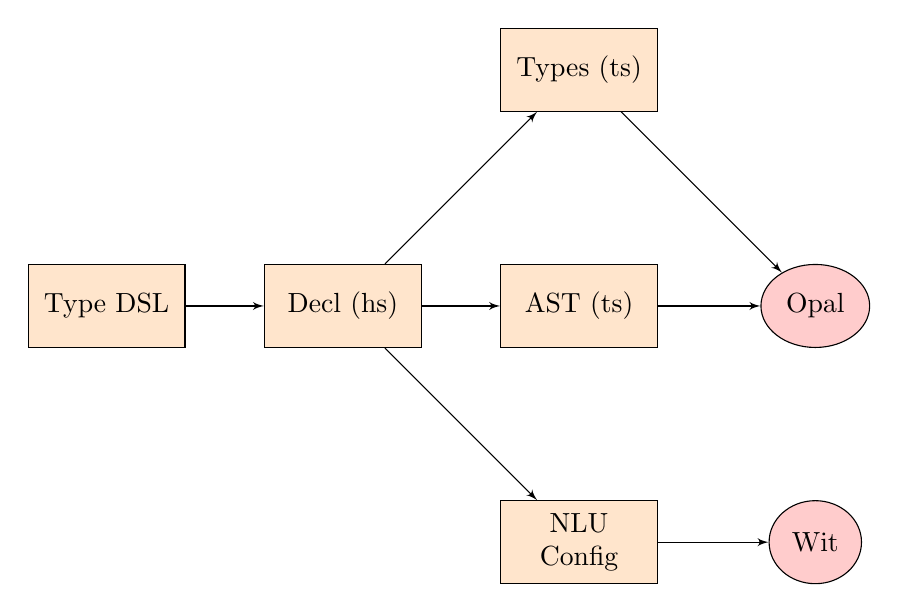
\begin{tikzpicture}[node distance = 3cm, auto]
    \node [block] (types) {Type DSL};
    \node [block, right of=types] (decls_hs) {Decl (hs)};
    \node [block, right of=decls_hs] (decls_ts) {AST (ts)};
    \node [block, below of=decls_ts] (cfg) {NLU Config};
    \node [block, above of=decls_ts] (ts_types) {Types (ts)};
    \node [cloud, right of=decls_ts] (ts) {Opal};
    \node [cloud, right of=cfg] (backend) {Wit};

    \path [line] (types) -- (decls_hs);
    \path [line] (decls_hs) -- (decls_ts);
    \path [line] (decls_hs) -- (cfg);
    \path [line] (decls_hs) -- (ts_types);
    \path [line] (decls_ts) -- (ts);
    \path [line] (ts_types) -- (ts);
    \path [line] (cfg) -- (backend);
  \end{tikzpicture}
  \caption{The configuration process.}
  \label{fig:process}
\end{figure*}
A high-level workflow for our implementation is shown in Figure
\ref{fig:process}. The programmer writes types in our DSL and uses our Haskell
tool to parse the declarations. The tool serializes three artifacts: a set of
TypeScript type declarations, an AST datastructure, and a set of JSON
configuration files for Wit. The programmer simply imports the types and AST
into their Opal project, uploads the JSON files to Wit, and the system is ready
to go.

\subsection{Configuration Tool}
When a user wants to configure an Opal application to interact with an NLU
library like Wit, they begin by using our configuration tool. The tool ensures
that the NLU engine responses will agree with the type definitions in the user's
application.

Our configuration tool is written in Haskell, and is designed to be simple and
obviously correct. We use the Parsec library to parse the type DSL into the
intermediate representation mentioned in Figure \ref{fig:hs_ast}.\cite{parsec}

\begin{figure}[H]
\begin{minted}{haskell}
  data Decl = FreeText String
            | Keywords String
                       [String]
            | Trait String
                    [(String, Ty)]
            | Alias String Ty
            deriving (Show)

  data Ty = Def String
          | Lit String
          | Rec [(String, Ty)]
          deriving (Show)
\end{minted}
  \caption{The Haskell code for our AST.}
  \label{fig:hs_ast}
\end{figure}

After parsing with Parsec, we apply versions of the \ff{interp} and \ff{cfg}
functions from Section \ref{formalism} to generate the appropriate
configuration.

\subsection{Run-time Library}
At run-time, a typical application using NLU will go through a fairly consistent
cycle.
\begin{enumerate}
\item Ask user for input, converting voice to text if necessary.
\item Query the NLU engine and obtain a response for the given input.
\item Parse the response into application data.
\item Process parsed data, and repeat.
\end{enumerate}
Steps 1 and 4 are generally application-specific, so we have elected to provide
a library which handles steps 2 and 4. For each backend that Opal
supports,\footnote{At the time of writing, Wit is the only supported backend.}
we provide utilities for querying the API and parsing the response data. The
network code involved in obtaining the response is fairly uninteresting, so we
will focus on the parsing.

In section \ref{formalism}, we outline the parse function, which takes a
declaration and a response and generates an Opal object. The function that we
provide in the Opal library is similar, but there are two important differences.
First, the parse function takes some element of $\fcy{D}$, which it uses to
deduce the structure of the desired output. In the real application, the analog
of $\fcy{D}$ is the \hs{Decl} type in the Haskell code; this is not available to
the Opal application at run time.

We get around this by using a modified version the a TypeScript library called
Runtypes.\cite{runtypes} Runtypes allows us to to serialize declarations
directly into TypeScript and therefore to keep necessary information around at
run-time. We extend Runtypes to include a type for entities---which map to
declarations in $\fcy{D}$. Runtypes provides the infrastructure for non-entity
types in $\fcy{T}$.

The other difference arises because Opal does not have dependent types. We
cannot completely faithfully transcribe the \ff{parse} function from above,
because it is not obvious that it can be typed at all. The solution here is to
combine Opal's dynamic typing with Runtypes' dynamic checking feature to create
a function that appears to be dependently typed. First, we use dynamic types
within the \ff{parse}. While building a response object, we assume, where
necessary, that it has type \ts{any}. Then, once parsing is complete, we use the
Runtypes object to check the parsed result, and we cast the result to the
desired type. The definition is shown in Figure \ref{fig:parse}. The cast is
safe, so long as the user respects the invariant that parse is always called
with compatible type and runtype parameters.

\begin{figure*}
\begin{minted}{typescript}
            public parse<T>(rt: Runtype<any>, res: Response): T {
                return rt.check(this._parse(rt, res)) as T;
            }

            private _parse(rt: Runtype<any>, res: Response): any { ... }
\end{minted}
  \caption{The wit parse functions.}
  \label{fig:parse}
\end{figure*}

\section{Evaluation} \label{evaluation}
Working with the system to build some toy applications led us to a number of
important conclusions about its effectiveness. We discuss a number of these
conclusions here.

\subsection{Type Expressiveness}
The first important thing we found when starting to write types in our DSL is
that the standard three entity types are not quite expressive enough for real
applications. For example, when trying to implement a small chatbot for
scheduling calendar meetings, we wanted to write something like,
\begin{minted}{typescript}
  free-text Person
  ...
  trait Intent = <Schedule> {
    person: Person,
    date: Date,
    time: Time
  }
\end{minted}
but we found that we had no way to express a date or a time. Technically
speaking, it might have been possible to encode dates and times as free text and
do a second parsing pass in the application code, but that solution is far from
elegant. We discuss one potential solution to this problem in Section
\ref{future>types}.

\subsection{Programmer Freedom}
When working around unsupported types, there is an obvious tendency to modify
the application types to better fit the capabilities of the system. It turns out
that this occurs in more cases than just using dates and times. For example,
consider a different set of types for calendar scheduling.
\begin{minted}{typescript}
keywords WkDay = "Sunday" | ...
alias Abs = {
  day: WkDay
  person: Person
}
keywords RDay = "today" | "tomorrow"
alias Rel = {
  day: RDay
  person: Person
}
trait Intent =
  | <Absolute> Abs
  | <Relative> Rel
\end{minted}
Here, we've done away with the complications of dates and times, and we just
allow a user to specify a day of the week or a ``relative day.'' The interesting
observation here is that this is likely not the way that most TypeScript/Opal
developers would write that type. For example, one reasonable alternative might
express days as a top-level disjunction, and then make the type of intents a
normal record.
\begin{minted}{typescript}
  type Day =
    | { tag: "today" }
    | { tag: "tomorrow" }
    | { tag: "abs", day: WkDay }
  type Intent =
    { day: Day, person: Person }
\end{minted}
This makes sense, since \ts{Absolute} and \ts{Relative} are not actully
different \emph{intents}, per se. We can see that the system has led us to a
different type than we would normally write.

It turns out that this might actually be a good thing, if viewed from the
perspective of the NLU engine itself. While \ts{Absolute} and \ts{Relative} are
the same intent from a philosophical perspective, they might be parsed very
differently. The utterance
\begin{center}
  \emph{Schedule my Wednesday meeting with Alice.}
\end{center}
is very different in structure from
\begin{center}
  \emph{Set a meeting with Bob tomorrow.}
\end{center}
Thus, it might be the case that forcing the programmer to write slightly
different types will make it much easier for the NLU backend to find the correct
information. There is likely some work to be done in terms of making our types
more idiomatic, but for now we err on the side of making life easier for the NLU
engine.

\subsection{Relative Success}
There is still a lot to be done on this work and in this space, but as of
writing, we feel that we have proven the concept fairly well. The system does
the job it intends to, and is usable for actual applications. In general, using
the tools feels fairly natural. The Haskell tool produces the output that a user
would expect, and the programming interface provides the functionality that a
user needs to actually write an application that uses NLU. Overall, we are happy
with our approach to the stated problem as well as with the results of the
implementation.

\section{Future Work} \label{future}
Moving forward, we hope to take this work in two main directions---wider support
for NLU features and backends and entirely new features.

\subsection{Wider Support}
Expanding support for more entity types and backends is an obvious way to
increase the usefulness of our work. Here, we discuss both of those extensions
in detail.

\subsubsection{More Types} \label{future>types}
In addition to the three ``universal'' kinds of entities (free text, keywords,
and traits), the Wit NLU engine provides more specialized ways of looking up
entities. Wit provides support for parsing numbers, dates, times, and other
specific forms of text. We elected to keep things simple at first and exclude
these built-in entities, but adding support for them seems like a very
reasonable next-step.

At a first approximation, this would require modifying the definitions of
$\fcy{D}$ and $\tau$ to include declarations for built-in entities and
base types for the data associated with those entities. More work needs to be
done exploring this space before any more specific conclusions can be drawn.

\subsubsection{More Backends}
We are also interested exploring NLU engines beyond Wit. One reason for this is
purely practical---users might want to use other backends, and it would be nice
for Opal to support this. Another reason, however, is more academic. Exploring
other NLU engines would give us opportunities to test the generality of our
current design. Preliminary research suggests that building our type system
around entities and search strategies makes sense, but we can only know that for
sure if we try to build interfaces for more engines.

\subsection{Interesting Features}
There are a number of novel research directions available as extensions to this
project. The following are two of the many ideas that we have had.

\subsubsection{Confidence-Based Parsing}
Up to this point, we have assumed very little about the data returned in the NLU
response. In practice, however, many NLU engines provide more than just
information about the matched entities. Wit, in particular, provides confidence
levels for each entity that it finds. Thus, a value like \ts{"Set"} might be
paired with a confidence level of $70\%$, meaning that Wit is $70\%$ sure that
the user's intent is actually to set a new reminder.

As of now, we do not actually use this information. In the majority of cases
that we have tested, a Wit bot either has enough information to get the right
entities, or it does not. However, it is possible that as we attempt to support
new types of entities and as user types get more complicated, it will be useful
to try multiple parses of a single response. In that case, we can choose between
different parses using confidence scores.

\subsubsection{Training with Tests}
A final extension of this project would attempt to close the code/configuration
gap even further by allowing users to train their NLU application in a way that
is guaranteed to support their tests. We would accomplish this using the same
idea behind our type DSL---we introduce a new DSL (or an extension to the
current one) for generating both Wit training examples and application tests.
While synchronization is less of an issue with training than it is with
configuration, it would still be extremely convenient to express the entirety of
the application's behavior in one place.

Exploring this path would require a fair amount of implementation work, but we
would also need to take great care to avoid overfitting. It is unclear to what
extent this would become an issue.

\section{Conclusion} \label{conclusion}
The Opal langauge hopes to be the ideal language for building modern
applications that leverage machine learning techniques. As NLU becomes more and
more popular as a user interface, it makes sense that Opal would provide a clean
and safe interface for natural langauge interaction. This work contributes a
real, working tool in the Opal ecosystem that provides a first attempt at such
an interface.

As we move towards a future where the majority of our interactions with
computers happen via human language, projects like this will become more and
more important. It may be that the approach put forth in the paper paves the way
for safe, correct applications that work with NLU. However, even if a different
approach wins out, it is almost certain that safe interfaces to NLU engines will
eventually become wide-spread. Just as companies have tended to favor strongly
typed language for applications where correctness matters, programmers working
with NLU will eventually see the need to do so in a principled way.

\bibliography{paper}{}
\bibliographystyle{plain}

\end{document}